\ifdefined\COMPLETE
\else
    \input{./preambule-sacha-utf8.ltx}
    \begin{document}
\fi


\section{Probabilités conditionnelles}

\subsection{Introduction}

\subsubsection{Exemple introductif}

On considère la répartition suivante : \\

%% IL Y A UN MÉLANGE ENTRE FILLES ET GARÇONS ENTRE LE TABLEAU ET L'ARBRE... A CORRIGER

\begin{tabular}{|c|c|c|c|c|}
\hline
Classes de Terminales & L & ES & S & Total \\
\hline
Filles & 20 & 15 & 15 & 50 \\
\hline
Garçons & 12 & 25 & 30 & 67 \\
\hline
Total & 32 & 40 & 45 & 117 \\
\hline
\end{tabular}

\vspace*{.3cm}

\begin{itemize}
\item[•] On a $p_F\left(L\right) = \dfrac{20}{50}$. \\

On vérifie grâce à la définition : \\

$\dfrac{p\left(F\cap L\right)}{p\left(F\right)} = \dfrac{\dfrac{20}{117}}{\dfrac{50}{117}} = \dfrac{20}{117} \times \dfrac{117}{50} = \dfrac{20}{50}$. \\

\item[•] De même, on a $p_S\left(G\right) = \dfrac{30}{45}$. \\

On vérifie grâce à la définition : \\

$\dfrac{p\left(S\cap G\right)}{p\left(S\right)} = \dfrac{\dfrac{30}{117}}{\dfrac{45}{117}} = \dfrac{30}{117} \times \dfrac{117}{45} = \dfrac{30}{45}$.  
\end{itemize}

\newpage

\subsubsection{Définition}

Soit $\Omega$ un espace probabilisé fini. \\
Soient $A$ et $B$ deux événements de $\Omega$ tel que $p\left(A\right) \neq 0$. \\

La probabilité de l'événement $B$ sachant que l'événement $A$ est réalisé est donnée par la formule : \\

$p_A\left(B\right) = \dfrac{p\left(A \cap B\right)}{p\left(A\right)}$. \\

On a donc $p\left(A \cap B\right) = p\left(A\right) \times p_A\left(B\right)$. \\

\textbf{Remarque :} $p_A\left(B\right)$ est lu « p de B sachant A ».

\subsubsection{Exemples}

\textbf{Exemple n°1} 

Soit un jeu de 52 cartes. \\

On tire successivement deux cartes sans remise. \\

Soit l'événement A : « On tire deux piques ». \\

D'après l'exercice n°3 de la partie 1.5.2, on sait que $p\left(A\right) = \dfrac{1}{17}$. \\

Soit l'événement B : « La première carte tirée est un pique ». \\
Soit l'événement C : « La seconde carte tirée est un pique ». \\

On a $A = B \cap C$. \\
D'où $p\left(A\right) = p\left(B\cap C\right) = p\left(B\right) \times p_B\left(C\right) = \dfrac{13}{52} \times \dfrac{12}{51} = \dfrac{1}{17}$. \\

Les résultats sont cohérents. \\

\textbf{Exemple n°2} 

Soit une urne avec $5$ boules rouges et $1$ boule noire. \\ On tire une boule. \\

Soit l'événement A : « Il faut successivement tirer $3$ boules sans remise pour tirer la boule noire ». \\
Soit l'événement B : « La première boule tirée est rouge ». \\
Soit l'événement C : « La deuxième boule tirée est rouge ». \\
Soit l'événement D : « La troisième boule tirée est noire ». \\

On a $A = B \cap C \cap D$. \\

Ainsi $p\left(A\right)$ $=$ $p\left[\left(B\cap C\right) \cap D\right]$ $=$ $p\left(B \cap C\right) \times p_{B \cap C}\left(D\right)$. \vspace*{.3cm} \\

En appliquant à nouveau la définition, on a $p\left(A\right) = p\left(B\right) \times p_B\left(C\right) \times p_{B\cap C}\left(D\right)$ $=$ $\dfrac{5}{6} \times \dfrac{4}{5} \times \dfrac{1}{4}$. \vspace*{.3cm} \\

D'où $p\left(A\right) = \dfrac{1}{6}$. 

\vspace*{-5cm}

\newpage

\vspace*{-1.5cm}

\textbf{Exemple n°3} 

Soient deux urnes $H$ et $K$. On sait que : \\

\begin{itemize}
\item[•] Dans $H$ : il y a $3$ boules rouges et $2$ boules vertes. 
\item[•] Dans $K$ : il y a $5$ boules rouges et $1$ boules verte. 
\end{itemize}

\vspace*{.3cm}

On jette un dé. Si on obtient un $1$ ou un $2$, on tire une boule de $H$. Sinon, on tire une boule de $K$. \\

Soit l'événement $A$ : « la boule tirée est verte ». \\
Soit l'événement $B$ : « la boule tirée vient de $H$ ». \\

\begin{itemize}
\item[1.] Déterminer la probabilité que la boule tirée soit verte. 
\item[2.] Sachant que la boule tirée est verte, quelle est la probabilité qu'elle vienne de $H$ ? 
\end{itemize}

\vspace*{.3cm}

\begin{itemize}
\item[1.] On cherche $p\left(A\right)$. \\
On a $A = \left(A \cap B\right) \cup \left(A \cap \overline{B}\right)$, avec $A \cap B$ et $A \cap \overleftarrow{B}$ deux événements incompatibles (cf le dessin suivant). \\


\centerline{
\begin{tikzpicture}
    \draw[color=red,thick] (0,0) circle (2cm) ; 
    \draw [red] (.5, 1.5) node {\large $\Omega$} ;
    \draw (0.5cm,0.2cm) circle (0.75cm) node [right] {\large $B$};
   \draw[color=green!70!black,pattern=north east lines] (-0.5cm,-0.3cm) circle (0.75cm) node[left] {\large $A$};
    \begin{scope}
    \clip (0.5cm,0.2cm) circle (0.75cm);
    \fill[fill=green!20] (-0.5cm,-0.3cm) circle (0.75cm);
    \end{scope}
    \pattern[color=green!20] (2.125cm,-1.5cm) rectangle +(0.5cm,0.5cm);
    \node[right] at (3cm,-1.25cm) {= $A \cap B$};
    \pattern[color=green!70!black,pattern=north east lines] (2.125cm,-2.5cm) rectangle +(0.5cm,0.5cm);
    \node[right] at (3cm,-2.25cm) {= $A \cap \overline{B}$};
    \end{tikzpicture}
}

\begin{tabular}{lll}
\hspace*{-.3cm} On a ainsi $p\left(A\right)$ & $=$ & $p\left[\left(A \cap B\right) \cup \left(A \cap \overline{B}\right)\right]$ \\
& $=$ & $p\left(A\cap B\right) \times p\left(A \cap \overleftarrow{B}\right)$ \\
& $=$ & $p\left(B \cap A\right) \times p\left(\overline{B} \cap A\right)$ \\
& $=$ & $p\left(B\right) \times p_B\left(A\right) + p\left(\overline{B}\right) \times p_{\overline{B}}\left(A\right)$ \\
& $=$ & $\dfrac{2}{6} \times \dfrac{2}{5} + \dfrac{4}{6} \times \dfrac{1}{6}$ \vspace*{.3cm} \\
& $=$ & $\dfrac{11}{45}$ \\
\end{tabular}

\vspace*{.3cm}

\item[2.] On cherche maintenant $p_A\left(B\right)$. \\

\begin{tabular}{lll}
\hspace*{-.3cm} On a $p_A\left(B\right)$ & $=$ & $\dfrac{p\left(A \cap B\right)}{p\left(A\right)}$ \vspace*{.3cm} \\
& $=$ & $\dfrac{p\left(B \cap A\right)}{p\left(A\right)}$ \vspace*{.3cm} \\
& $=$ & $\dfrac{p\left(B\right) \times p_B\left(A\right)}{p\left(A\right)}$ \vspace*{.3cm} \\
& $=$ & $\dfrac{\dfrac{2}{6} \times \dfrac{2}{5}}{\dfrac{11}{45}}$ \vspace*{.3cm} \\
& $=$ & $\dfrac{6}{11}$ \\
\end{tabular}

\vspace*{.3cm}

D'où $p_A\left(B\right) = \dfrac{6}{11}$.

\vspace*{-20cm}
\end{itemize}

\vspace*{-20cm}

\newpage

\vspace*{-1.5cm}

\subsection{Probabilités totales}

\subsubsection{Système complet d'événements}

Soit $\Omega$ un espace probabilité fini. \\
Soient $A_1, A_2, A_3, ..., A_n$ $n$ événements de $\Omega$. \\

On dit que $A_1, A_2, A_3, ..., A_n$ forme un \underline{système complet d'événements} de $\Omega$, ou une \underline{partition} de $\Omega$ \\ si et seulement si : \\

\begin{itemize}
\item[1.] Aucun des événements $A_1, A_2, A_3, ..., A_n$ n'est vide. 
\item[2.] L'intersection de deux événements quelconques des événements $A_1, A_2, A_3, ..., A_n$ est vide. 
\item[3.] La réunion des événements $A_1, A_2, A_3, ..., A_n$ est égale à $\Omega$. 
\end{itemize}

\vspace*{.3cm}

On donne l'exemple de représentation suivant : \\

\begin{tikzpicture}[line cap=round,line join=round,>=triangle 45,x=1.0cm,y=1.0cm,scale=.6]
\clip(2,.5) rectangle (13,9);
% \draw (2,1) -- (13,1) -- (13,9) -- (2,9) ; 
\draw [rotate around={21.9:(7.35,4.81)}] (7.35,4.81) ellipse (4.47cm and 3.19cm);

\draw [shift={(3.98,7.76)}] plot[domain=-1.85:0.1,variable=\t]({1*3.23*cos(\t r)+0*3.23*sin(\t r)},{0*3.23*cos(\t r)+1*3.23*sin(\t r)});
\draw [shift={(8.22,8.25)}] plot[domain=4.11:6,variable=\t]({1*2.55*cos(\t r)+0*2.55*sin(\t r)},{0*2.55*cos(\t r)+1*2.55*sin(\t r)});
\draw [shift={(12.16,6.14)}] plot[domain=3.25:4.23,variable=\t]({1*3.24*cos(\t r)+0*3.24*sin(\t r)},{0*3.24*cos(\t r)+1*3.24*sin(\t r)});
\draw [shift={(2.08,2.99)}] plot[domain=-0.26:0.59,variable=\t]({1*5.66*cos(\t r)+0*5.66*sin(\t r)},{0*5.66*cos(\t r)+1*5.66*sin(\t r)});
\draw [shift={(2.19,2.95)}] plot[domain=-0.43:0.55,variable=\t]({1*3.33*cos(\t r)+0*3.33*sin(\t r)},{0*3.33*cos(\t r)+1*3.33*sin(\t r)});
\draw (4.8,6.44) node[anchor=north west] {\Large $A_1$};
\draw (8,7.34) node[anchor=north west] {\Large $A_2$};
\draw (10,5.72) node[anchor=north west] {\Large $A_3$};
\draw (8.2,4.4) node[anchor=north west] {\Large $A_4$};
\draw (6,3.58) node[anchor=north west] {\Large $A_5$};
\draw (4,3.68) node[anchor=north west] {\Large $A_6$};
\end{tikzpicture}

\textbf{Remarque :} $A$ et $\overline{A}$ forment un système complet d'événements.

\subsubsection{Formule des probabilités totales}

Soit $\Omega$ un espace probabilité fini. \\
Soient $A_1, A_2, A_3, ..., A_n$ un système complet d'événements de $\Omega$. \\
Soit $B$ un événement quelconque de $\Omega$. \\

On a $B = \left(A_1 \cap B\right) \cup \left(A_2 \cap B\right) \cup \left(A_3 \cap B\right) \cup ... \cup \left(A_n \cap B\right) = \displaystyle\bigcup_{i=1}^n \; \left(A_i \cap B\right)$, \\ où $A_1 \cap B$, $A_2 \cap B$, $A_3 \cap B$, ... $A_n \cap B$ sont incompatibles. \\

On a la représentation ci-contre : 

\begin{tikzpicture}[line cap=round,line join=round,>=triangle 45,x=1.0cm,y=1.0cm]
\clip (4.5,3) rectangle (9.5,8) ; 
% \draw (4.5,3) rectangle (9.5,8) ;  

\draw [rotate around={40:(7,5.5)},blue] (7,5.5) ellipse (2.25cm and 1.9cm); % Tracé de Omega

\begin{scope} % On ne dessine qu'a l'intérieur de Omega
  \clip [rotate around={40:(7,5.5)}] (7,5.5) ellipse (2.25cm and 1.9cm) ;
    \draw [rotate around={-50:(7.1,5.9)},color=red,pattern=bricks, pattern color=red] (7.1,5.9) ellipse (1.3cm and 1cm);
    \draw [rotate around={70:(8,5)},line width=1.2pt,color=Blue,fill=white,fill opacity=0.25] (8,5) ellipse (1.5cm and 1.1cm); % A3
    \begin{scope} \clip [rotate around={70:(8,5)}] (8,5) ellipse (1.5cm and 1.1cm);
    \draw [rotate around={-50:(7.1,5.9)},color=red,color=red,pattern=north east lines, pattern color=red] (7.1,5.9) ellipse (1.3cm and 1cm);
    \end{scope}
    \draw [rotate around={-30:(8,7)},blue,line width=1.2pt,fill=white,fill opacity=0.5] (8,7) ellipse (2cm and 1cm); % A2   
    
    \begin{scope} \clip [rotate around={-30:(8,7)}] (8,7) ellipse (2cm and 1cm);
        \draw [rotate around={-50:(7.1,5.9)},color=red,pattern=vertical lines, pattern color=red] (7.1,5.9) ellipse (1.3cm and 1cm);
    \end{scope}
  
    \draw [rotate around={30:(6,7)},blue,line width=1.2pt,fill=white] (6,7) ellipse (1.7cm and 0.75cm); % A1
    
    \begin{scope} \clip [rotate around={30:(6,7)}] (6,7) ellipse (1.7cm and 0.75cm);
     \draw [rotate around={-50:(7.1,5.9)},color=red,pattern=dots, pattern color=red] (7.1,5.9) ellipse (1.3cm and 1cm);
    \end{scope}

\draw [rotate around={-50:(7.1,5.9)},color=red,line width=1.2pt] (7.1,5.9) ellipse (1.3cm and 1cm);
\draw [rotate around={40:(7,5.5)},blue,line width=1.2pt] (7,5.5) ellipse (2.25cm and 1.9cm); % On retrace Omega

 \end{scope} % Fin global 
 
 \draw [blue] (5.7,6.4) node {\large $A_1$} ; 
 \draw [blue] (8.3,6.8) node {\large $A_2$} ; 
 \draw [blue] (8.2,4.5) node {\large $A_3$} ; 
  \draw [blue] (6,4.5) node {\large $A_4$} ; 
\end{tikzpicture}

\begin{tabular}{lll}
\hspace*{-.3cm} On en déduit que $p\left(B\right)$ & $ = $ & $p\left[\left(A_1 \cap B\right) \cup \left(A_1 \cap B\right) \cup \left(A_1 \cap B\right) \cup ... \cup \left(A_1 \cap B\right)\right]$ \\
& $=$ & $p\left(A_1\cap B\right) + p\left(A_2 \cap B\right) + p\left(A_3 \cap B\right) + ... + p\left(A_n \cap B\right)$ \\
& $=$ & $p\left(A_1\right) \times p_{A_1}\left(B\right) + p\left(A_2\right) \times p_{A_2}\left(B\right) + p\left(A_3\right) \times p_{A_3}\left(B\right) + ... + p\left(A_n\right) \times p_{A_n}\left(B\right)$. \\
\end{tabular}

\vspace*{-5cm}

\newpage

\subsubsection{Exemple}

Sylvain possède un jeu électronique. \\ Une partie consiste en un duel entre Sylvain et un monstre choisi par la machine. \\

Deux choix équiprobables sont possibles : la machine choisi entre $4$ montres $M_1$ ou le monstre $M_2$. Les deux montres sont de force inégale. On admet que si Sylvain combat $M_1$, la probabilité qu'il gagne est de $\dfrac{1}{3}$. De plus, s'il combat $M_2$, la probabilité qu'il gagne est de $\dfrac{1}{4}$. \\

Soit $G$ l'événement : « Sylvain gagne ». \\
Soit $M_1$ l'événement : « La machine choisi le monstre $M_1$ ». \\
Soit $M_2$ l'événement : « La machine choisi le monstre $M_2$ ». \\

Déterminer $p\left(G\right)$. \\

D'après le texte, on a : \\

\begin{itemize}
\item[•] $p\left(M_1\right) = p\left(M_2\right) = \dfrac{1}{2}$. \\
\item[•] $p_{M_1}\left(G\right) = \dfrac{1}{3}$. \\
\item[•] $p_{M_2}\left(G\right) = \dfrac{1}{4}$. \\
\end{itemize}

On a $G = \left(G \cap M_1\right) \cup \left(G \cap M_2\right)$. \\

De plus, $M_1$ et $M_2$ forme un système complet d'événements (en fait, $M_2 = \overline{M_1}$). \\

Ainsi, d'après la formule des probabilités totales, on a : \\

\begin{tabular}{lll}
$p\left(G\right)$ & $=$ & $p\left[ \left(G \cap M_1\right) \cup \left(G \cap M_2\right) \right]$ \vspace*{.3cm} \\
& $=$ & $p\left(G\cap M_1\right) + p\left(G \cap M_2\right)$ \vspace*{.3cm} \\
& $=$ & $p\left(M_1 \cap G\right) + p\left(M_2 \cap G\right)$ \vspace*{.3cm} \\
& $=$ & $p\left(M_1\right) \times p_{M_1}\left(G\right) + p\left(M_2\right) \times p_{M_2}\left(G\right)$ \vspace*{.3cm} \\
& $=$ & $\dfrac{1}{2} \times \dfrac{1}{3} + \dfrac{1}{2} \times \dfrac{1}{4}$ \vspace*{.3cm} \\
& $=$ & $\dfrac{7}{24}$.
\end{tabular}

\vspace*{.3cm}

Ainsi la probabilité que Sylvain gagner sa partie est de $\dfrac{7}{24}$. 

\newpage

\subsubsection{Exercices}

\textbf{Exercice n°1} \\

À la cafétéria, dans une vitrine pâtisserie : \\

\begin{itemize}
\item[•] $60 \;$ \% des gâteaux sont à base de crème ;
\item[•] parmi ceux qui sont à base de crème, $35 \;$ \% ont aussi des fruits ; 
\item[•] parmi les gâteaux qui n'ont pas de crème, $85 \;$ \% ont des fruits. 
\end{itemize}

\vspace*{.3cm}

On prend un gâteau au hasard. \\

\begin{itemize}
\item[1.]
\begin{itemize}
\item[a)] Calculer la probabilité d'avoir un gâteaux à base de crème et comportant des fruits. 
\item[b)] Calculer la probabilité d'avoir un gâteau avec des fruits mais sans crème.
\item[c)] En déduire la probabilité d'avoir un gâteaux avec des fruits. \\
\end{itemize}
\item[2.]
\begin{itemize}
\item[a)] La gâteau pris au hasard comporte des fruits.\\ Quelle est la probabilité qu'il soit à base de crème ?
\item[b)] Le gâteau pris au hasard ne comporte pas de fruit. \\ Quelle est la probabilité qu'il soit à base de crème ?
\end{itemize}
\end{itemize}

\vspace*{.3cm}

\textbf{Solution} \\

Soit $C$ l'événement : « Le gâteau est à la crème. » \\
Soit $F$ l'événement : « Le gâteau compte des fruits. » \\

D'après le texte : \\

\begin{itemize}
\item[•] $p\left(C\right) = \dfrac{3}{5}$ \vspace*{.3cm} \\
\item[•] $p_C\left(F\right) = \dfrac{7}{20}$, on en déduit que $p_C\left(\overline{F}\right) = \dfrac{13}{20}$ \vspace*{.3cm} \\
\item[•] $p_{\overline{C}}\left(F\right) = \dfrac{17}{20}$ \vspace*{.3cm} \\
\end{itemize}


\begin{itemize}
\item[1.] 
\begin{itemize}
\item[a)] On cherche $p\left(C \cap F\right)$. \\

On a $p\left(C\cap F\right) = p\left(C\right) \times p_C\left(F\right)$. \\

D'où $p\left(C \cap F\right) = \dfrac{3}{5} \times \dfrac{7}{20} = \dfrac{21}{100}$. \\

\item[b)] On cherche $p\left(F \cap \overline{C}\right)$. \\

On a $p\left(F \cap \overline{C}\right) = p\left(\overline{C} \cap F\right) = p\left(\overline{C}\right) \times p_{\overline{C}}\left(F\right)$. \\

D'où $p\left(F \cap \overline{C}\right) = \dfrac{2}{5} \times \dfrac{17}{20} = \dfrac{34}{100} = \dfrac{17}{50}$. \\

\newpage

\item[c)] On cherche $p\left(F\right)$. \\

On a $F = \left(F \cap C\right) \cup \left(F \cap \overline{C}\right)$. \\

$C$ et $\overline{C}$ forment un système complet d'événements. \\

\begin{tabular}{lll}
\hspace*{-.3cm} Ainsi $p\left(F\right)$ & $=$ & $p\left[\left(F \cap C\right) \cup \left(F \cap \overline{C}\right)\right]$. \\
& $=$ & $p\left(F \cap C\right) + p\left(F \cap \overline{C}\right)$. 
\end{tabular}

\vspace*{.3cm}

D'après la question 1.a), on a $p\left(F \cap C\right) = \dfrac{21}{100}$. \\

D'après la question 1.b), on a $p\left(F \cap \overline{C}\right) = \dfrac{17}{50}$. \\

D'où $p\left(F\right) = \dfrac{21}{100} + \dfrac{17}{50}  = \dfrac{55}{100} = \dfrac{11}{20}$. \\

\end{itemize}
\item[2.] 
\begin{itemize}
\item[a)] On cherche $p_F\left(C\right)$. \\

\begin{tabular}{lll}
\hspace*{-.3cm} Par définition, $p_F\left(C\right)$ & $=$ & $\dfrac{p\left(F \cap C\right)}{p\left(F\right)}$. \vspace*{.3cm} \\
& $=$ & $\dfrac{p\left(C\cap F\right)}{p\left(F\right)}$. \vspace*{.3cm} \\
& $=$ & $\dfrac{p\left(C\right) \times p_C\left(F\right)}{p\left(F\right)}$. 
\end{tabular}

\vspace*{.3cm}

Ainsi $p_F\left(C\right) = \dfrac{\dfrac{3}{5} \times \dfrac{7}{20}}{\dfrac{11}{20}} = \dfrac{21}{55}$. \\

\item[b)] On cherche $p_{\overline{F}}\left(C\right)$. \\

\begin{tabular}{lll}
\hspace*{-.3cm} Par définition, $p_{\overline{F}}\left(C\right)$ & $=$ & $\dfrac{p\left(\overline{F} \cap C\right)}{p\left(\overline{F}\right)}$. \vspace*{.3cm} \\
& $=$ & $\dfrac{p\left(C\cap \overline{F} \right)}{p\left(\overline{F}\right)}$. \vspace*{.3cm} \\
& $=$ & $\dfrac{p\left(C\right) \times p_C\left(\overline{F}\right)}{p\left(\overline{F}\right)}$. 
\end{tabular}

\vspace*{.3cm}

Ainsi $p_{\overline{F}}\left(C\right) = \dfrac{\dfrac{3}{5} \times \dfrac{13}{20}}{\dfrac{9}{20}} = \dfrac{13}{15}$. \\
\end{itemize}
\end{itemize}

\newpage

\textbf{Exercice n°2} \\

Un stock de champignons est constitué de trois variétés de champignons conditionnés en barquettes. Ces barquettes proviennent exclusivement de France ou d'Italie. \\

Ce stock est composé à $50 \;$ \% de barquettes de cèpes, à $30 \;$ \% de barquettes de girolles et à $20 \;$ \% de barquettes de morilles. \\

On sait que : \\

\begin{itemize}
\item[•] $15 \;$ \% des barquettes de cèpes proviennent d'Italie. 
\item[•] $20 \;$ \% des barquettes de girolles proviennent d'Italie. 
\item[•] $40 \;$ \% des barquettes de morilles proviennent d'Italie. 
\end{itemize}

\vspace*{.3cm}

On choisit une barquette au hasard. On notera les événements suivants : \\

\begin{itemize}
\item[•] $C$ : « La barquette choisie contient des cèpes . » 
\item[•] $G$ : « La barquette choisie contient des girolles . » 
\item[•] $M$ : « La barquette choisie contient des morilles . » 
\item[•] $I$ : « La barquette choisie provient d'Italie. » 
\item[•] $F$ : « La barquette choisie provient de France. » 
\end{itemize}

\vspace*{.3cm}

\begin{itemize}
\item[1.] On construira l'arbre de probabilités associé au problème. \\

\item[2.] Quelle est la probabilité que la barquette choisie contienne des cèpes et provienne de France ? \\

\item[3.] Quelle est la probabilité que la barquette choisie provienne d'Italie ? \\

\item[4.] Quelle est la probabilité que la barquette choisie contienne des cèpes sachant que cette barquette provient d'Italie ? On donnera une valeur arrondie à $10^{-3}$. \\

\item[5.] La barquette choisie provient de France. Quelle est la probabilité que ce soit une barquette de girolles ? On donnera une valeur arrondie à $10^{-3}$. 
\end{itemize}

\vspace*{.3cm}

\textbf{Solution} \\

D'après le texte : \\

\begin{itemize}
\item[•] $p\left(C\right) = \dfrac{1}{2}$. \\
\item[•] $p\left(G\right) = \dfrac{3}{10}$. \\
\item[•] $p\left(M\right) = \dfrac{1}{5}$. \\
\item[•] $p_C\left(I\right) = \dfrac{3}{20}$. \\
\item[•] $p_G\left(I\right) = \dfrac{1}{5}$. \\
\item[•] $p_M\left(I\right) = \dfrac{2}{5}$. 
\end{itemize}

\newpage

%\vspace*{-.3cm}

\begin{itemize}
\item[1.] On a l'arbre de probabilités suivant : \vspace*{.3cm} \\

\begin{tikzpicture}                                                                                       
  \tikzstyle{level 1}=[level distance=2cm, sibling distance=2cm]
  \tikzstyle{level 2}=[level distance=2cm, sibling distance=1cm]
                    
   \node{}[grow=right] % Pas de ligne blanche ci-dessous 
       child{node[blue]{$M$}                                                                               
                    child{node{$I$} edge from parent node[below,blue]{$\frac{2}{5}$}}              
                    child{node{$F$} edge from parent node[above,green]{$\frac{3}{5}$}}
                    edge from parent node[blue,below]{$\dfrac{1}{5}$}}                   
       child{node[blue]{$G$}
                    child{node{$I$} edge from parent node[below,blue]{$\frac{1}{5}$}}
                    child{node{$F$} edge from parent node[above,green]{$\frac{4}{5}$}}
                    edge from parent node[blue] {$\dfrac{3}{10}$}}                    
       child{node[blue]{$C$}
                    child{node{$I$} edge from parent node[below,blue]{$\frac{3}{20}$}}
                    child{node{$F$} edge from parent node[above,green]{$\frac{17}{20}$}}
                    edge from parent node[blue,above]{$\dfrac{1}{2}$}}                    
       
;
                    
\end{tikzpicture}

\vspace*{.6cm}

\item[2.] On cherche $p\left(C \cap F\right)$. \vspace*{.3cm} \\

On a $p\left(C \cap F\right) = p\left(C\right) \times p\left(F\right)$ car $C$ et $F$ sont indépendants. \vspace*{.3cm} \\

D'où $p\left(C\cap F\right) = \dfrac{1}{2} \times \dfrac{17}{20}$. \vspace*{.3cm} \\

Ainsi $p\left(C\cap F\right) = \dfrac{17}{40}$. \vspace*{.3cm} \\

\item[3.] On cherche $p\left(I\right)$. \vspace*{.3cm} \\

On a $I = \left(I \cap C\right) \cup \left(I \cap G\right) \cup \left(I \cap M\right)$. \vspace*{.3cm} \\

$C$, $G$ et $F$ forment un système complet d'événements, on peut donc appliquer la formule des probabilités totales. \\

\begin{tabular}{lll}
\hspace{-.3cm} Ainsi $p\left(I\right)$ & $=$ & $p\left[\left(I \cap C\right) \cup \left(I \cap G\right) \cup \left(I \cap M\right)\right]$ \vspace*{.3cm} \\
& $=$ & $p\left(I \cap C\right) + p\left(I \cap G\right) + p\left(I \cap M\right)$ \vspace*{.3cm} \\
& $=$ & $p\left(C\right) \times p_C\left(I\right) + p\left(G\right) \times p_G\left(I\right) + p\left(M\right) \times p_M\left(I\right)$ \vspace*{.3cm} \\
& $=$ & $\dfrac{1}{2} \times \dfrac{3}{20} + \dfrac{3}{10} \times \dfrac{1}{5} + \dfrac{1}{5} \times \dfrac{2}{5}$ \vspace*{.3cm} \\
& $=$ & $\dfrac{43}{200}$ \\
\end{tabular}

\newpage

\item[4.] On cherche $p_I\left(C\right)$. \vspace*{.3cm} \\

Par définition, $p_I\left(C\right) = \dfrac{p\left(I \cap C\right)}{p\left(I\right)}$. \vspace*{.3cm} \\

\begin{tabular}{lll}
\hspace*{-.3cm} D'où $p_I\left(C\right)$ & $ = $ & $ \dfrac{p\left(C \cap I\right)}{p\left(I\right)}$ \vspace*{.3cm} \\
& $=$ & $\dfrac{p\left(C\right) \times p_C\left(I\right)}{p\left(I\right)}$ \\
\end{tabular}

\vspace*{.6cm}

Donc $p_I\left(C\right) = \dfrac{\dfrac{1}{2} \times \dfrac{3}{20}}{\dfrac{43}{200}} = \dfrac{15}{43}$. \vspace*{.3cm} \\

D'où $p_I\left(C\right) \approx 0,349$. \vspace*{.3cm} \\

\item[5.] On cherche $p_F\left(G\right)$. \vspace*{.3cm} \\

Par définition, $p_F\left(G\right) = \dfrac{p\left(F \cap G\right)}{p\left(F\right)}$. \vspace*{.3cm} \\

\begin{tabular}{lll}
\hspace*{-.3cm} D'où $p_F\left(G\right)$ & $ = $ & $ \dfrac{p\left(G \cap F\right)}{p\left(F\right)}$ \vspace*{.3cm} \\
& $=$ & $\dfrac{p\left(G\right) \times p_G\left(F\right)}{p\left(F\right)}$ \\
\end{tabular}

\vspace*{.6cm}

On cherche $p_G\left(F\right)$. \vspace*{.3cm} \\

On a $p_G\left(F\right) = 1 - p_G\left(I\right) = 1 - \dfrac{1}{5} = \dfrac{4}{5}$. \vspace*{.3cm} \\

On cherche $p\left(F\right)$. \\

On a $p\left(F\right) = 1 - p\left(I\right) = 1 - \dfrac{43}{200} = \dfrac{157}{200}$. \vspace*{.3cm} \\

\begin{tabular}{lll}
\hspace*{-.3cm} D'où $p_F\left(G\right)$ & $=$ & $\dfrac{\dfrac{3}{10} \times \dfrac{4}{5}}{\dfrac{157}{200}}$. \vspace*{.3cm} \\
& $=$ & $\dfrac{48}{157}$ \\
\end{tabular}

\vspace*{.6cm}

Donc $p_F\left(G\right) \approx 0,306$.

\end{itemize}

\newpage

%\vspace*{-.5cm}

\textbf{Exercice n°3} \\

Dans un magasin, un acheteur potentiel s'intéresse à un lave-linge et un sèche-linge. \\

La probabilité qu'il achète le lave-linge est de $0,6$. \\
La probabilité qu'il achète le sèche-linge quand il a acheté le lave-linge est de $0,7$. \\
La probabilité qu'il achète le sèche-linge quand il n'a pas acheté le lave-linge est de $0,1$. \\

On désigne par $L$ l'événement : « le client achète le lave-linge » et par $S$ l'événement : « le client achète le sèche-linge ». \\

\begin{itemize}
\item[1.] Déterminer les probabilités des événements suivants : \\
\begin{itemize}
\item[a)] « Le client n'achète le lave-linge ». 
\item[b)] « Le client n'achète pas le sèche-linge quand il n'a pas acheté le lave-linge ». \\
\end{itemize}
\item[2.] Montrer que la probabilité que le client n'achète ni le lave-linge ni le sèche-linge est de $0,36$. \\
\item[3.] Le lave-linge coûte $400$ euros et le sèches-linge $320$ euros. \\ On désigne par $D$ la dépense du client. \\
\begin{itemize}
\item[a)] Établir les valeurs possibles de la variable aléatoire $D$.
\item[b)] Déterminer la loi de probabilité de $D$.
\item[c)] Calculer l'espérance mathématique de $D$.
\item[d)] Le « service clientèle » du magasin sait qu'il se présente en moyenne chaque semaine $25$ acheteurs potentiels pour ces deux appareils. Quel chiffre d'affaires hebdomadaire le magasin peut-il espérer réaliser ?
\end{itemize} 
\end{itemize}

\vspace*{.3cm}

\textbf{Solution} \\

D'après le texte : \\

\begin{itemize}
\item[•] $p\left(L\right) = 0,6$. \\
\item[•] $p_L\left(S\right) = 0,7$. \\
\item[•] $p_{\overline{L}}\left(S\right) = 0,1$. \\
\end{itemize}

\vspace*{.3cm}

\begin{itemize}
\item[1.]
\begin{itemize}
\item[a)] On cherche $p\left(\overline{L}\right)$. \\

\begin{tabular}{lll}
\hspace*{-.3cm} $p\left(\overline{L}\right)$ & $=$ & $1 - p\left(L\right)$ \\
& $=$ & $1 - 0,6$ \\
& $=$ & $0,4$ \\
\end{tabular}

\vspace*{.3cm}

\item[b)] On cherche $p_{\overline{L}}\left(\overline{S}\right)$. \\

\begin{tabular}{lll}
On a $p_{\overline{L}}\left(\overline{S}\right)$ & $=$ & $1 - p_{\overline{L}}\left(S\right)$ \\
& $=$ & $1 - 0,1$ \\
& $=$ & $0,9$. 
\end{tabular}
\end{itemize}

\vspace*{-5cm}

\newpage

\item[2.] On cherche $p\left(\overline{S} \cap \overline{L}\right)$. \\

\begin{tabular}{lll}
$p\left(\overline{S} \cap \overline{L}\right)$ & $=$ & $p\left(\overline{L} \cap \overline{S}\right)$ \\
& $=$ & $p\left(\overline{L}\right) \times p_{\overline{L}}\left(\overleftarrow{S}\right)$ \\
& $=$ & $0,4 \times 0,9$ \\
& $=$ & $0,36$ \\
\end{tabular}

\vspace*{.3cm}

\item[3.]
\begin{itemize}
\item[a)] On a $D\left(\Omega\right) = \lbb 0 \; ; \; 320 \; ; \; 400 \; ; \; 720 \rbb$. \\
\item[b)] On cherche à déterminer la loi de probabilité de $D$. \\

\begin{itemize}
\item[•] On a $p\left(\overline{L} \cap \overline{S}\right) = 0,36$. \vspace*{.3cm} \\
\item[•] De plus, $p\left(L \cap \overline{S}\right) = p\left(L\right) \times P_L\left(\overline{S}\right) = p\left(L\right) \times \left(1 - p_L\left(S\right)\right)$. \\

Ainsi $p\left(L \cap \overline{S}\right) = 0,6 \times \left(1 - 0,7\right) = 0,18$. \vspace*{.3cm} \\

\item[•] On a aussi $p\left(\overline{L} \cap S\right) = p\left(\overline{L}\right) \times p_{\overline{L}}\left(S\right) = 0,4 \times 0,1 = 0,04$. \vspace*{.3cm} \\

\item[•] Enfin, $p\left(L\cap S\right) = 1 - \left[p\left(\overline{L} \cap \overline{S}\right) + p\left(L \cap \overline{S}\right) + p\left(\overline{L} \cap S\right) \right]$. \\

Donc $p\left(L \cap S\right) = 1 - \left(0,36 + 0,18 + 0,04\right) = 0,42$. \\
\end{itemize}

\vspace*{.3cm}

On en déduit le tableau suivant, qui donne la loi de probabilités suivie par $D$ : \\

\begin{tabular}{c|c|c|c|c}
$x_i$ & $0$ & $320$ & $400$ & $720$ \\
\hline
$p\left(X = x_i\right)$ & $0,36$ & $0,18$ & $0,04$ & $0,42$ \\
\end{tabular}

\vspace*{.6cm}

\item[c)] On a $E\left(D\right) = 0 \times 0,36 + 320 \times 0,18 + 400 \times 0,04 + 720 \times 0,42$. \\

D'où $E\left(D\right) = 387,2$. \\

Ainsi, en moyenne, un client dépense $387,20$ euros dans le magasin. \\

\item[d)] Soit $CA$ le chiffre d'affaire cherché. \\

On a $CA = 25 \times E\left(D\right) = 25 \times 387,20 = 9680$. \\

Ainsi, le magasin peut espérer réaliser un chiffre d'affaire de $9680$ euros hebdomadaire.
\end{itemize}
\end{itemize}

\newpage

\textbf{Exercice n°4} \\

Une étude a été faite sur la fréquentation du cinéma dans une ville française pendant un mois. \\
Dans cette ville, $25 \;$ \% des habitants sont dans la tranche d'âge $0-14$ ans (les « enfants ») et $20 \;$ \% des habitants sont dans la tranche d'âge $15-25$ ans (les « jeunes »). Les autres habitants seront dits « adultes ». \\

On choisit un habitant dans cette ville au hasard. \\

On note $E$, $J$, $A$ les événements suivants : \\

\begin{itemize}
\item[•] $E$ : « L'habitant choisi est dans la tranche $0-14$ ans. »
\item[•] $J$ : « L'habitant choisi est dans la tranche $15-25$ ans. »
\item[•] $A$ : « L'habitant choisi est un adulte ». 
\end{itemize}

\vspace*{.3cm}

On appelle $X$ la variable aléatoire égale au nombre de séances auxquelles l'habitant choisi a assisté pendant un mois. \\

L'étude menée permet d'établir les tableaux de probabilités conditionnelles suivants : \\

\centerline{
\begin{tabular}{lll}
\hspace*{-.5cm} \begin{minipage}{5.5cm}
\begin{tabular}{|c|c|c|c|c|}
\hline
$x_i$ & $0$ & $1$ & $2$ & $3$ \\
\hline
& & & & \\
$P_E\left(X = x_i\right)$ & $\dfrac{3}{10}$ & $\dfrac{3}{10}$ & $\dfrac{2}{10}$ & $\dfrac{2}{10}$ \\
& & & & \\
\hline
\end{tabular}
\end{minipage}
&
\begin{minipage}{6.3cm}
\begin{tabular}{|c|c|c|c|c|c|}
\hline
$x_i$ & $0$ & $1$ & $2$ & $3$& $4$ \\
\hline
& & & & & \\
$P_J\left(X = x_i\right)$ & $\dfrac{1}{10}$ & $\dfrac{2}{10}$ & $\dfrac{3}{10}$ & $\dfrac{3}{10}$ & $\dfrac{1}{10}$ \\
& & & & & \\
\hline
\end{tabular}
\end{minipage}
&
\begin{minipage}{5cm}
\begin{tabular}{|c|c|c|c|c|}
\hline
$x_i$ & $0$ & $1$ & $2$ & $3$ \\
\hline
& & & & \\
$P_A\left(X = x_i\right)$ & $\dfrac{4}{10}$ & $\dfrac{3}{10}$ & $\dfrac{2}{10}$ & $\dfrac{1}{10}$ \\
& & & & \\
\hline
\end{tabular}
\end{minipage}
\\
\end{tabular}
}

\vspace*{.5cm}

Exemple : $p_J\left(X = 2\right)$ désigne la probabilité pour que l'habitant choisi aille deux fois par mois au \\ cinéma sachant qu'il est jeune. \\

\begin{itemize}
\item[1.] Déterminer la probabilité que l'habitant choisi : \\
\begin{itemize}
\item[a)] soit adulte.
\item[b)] soit jeune et aille deux fois par mois au cinéma. \\
\end{itemize}
\item[2.] Calculer la probabilité pour que l'habitant choisi aille deux fois par mois au cinéma. \\
\item[3.]
\begin{itemize}
\item[a)] Compléter le tableau suivant pour obtenir la loi de probabilité de la variable aléatoire $X$ : \\

\begin{tabular}{|c|c|c|c|c|c|}
\hline
$x_i$ & $0$ & $1$ & $2$ & $3$ & $4$ \\
\hline
$P\left(X = x_i\right)$ & $0,315$ & $0,280$ & \hspace*{.3cm} & \hspace*{.3cm} & \hspace*{.3cm} \\
\hline
\end{tabular}

\vspace*{.5cm}

\item[b)] Calculer l'espérance mathématique de $X$, notée $E\left(X\right)$. \\ Interpréter le résultat obtenu.

\end{itemize}
\end{itemize}

\newpage

\vspace*{-1.5cm}

\textbf{Solution} \\

D'après le texte : \\

\begin{tabular}{ll}
\begin{minipage}{6cm}
\begin{itemize}
\item[•] $\left(E\right) = \dfrac{1}{4}$.
\end{itemize}
\end{minipage}
&
\begin{minipage}{5cm}
\begin{itemize}
\item[•] $p\left(J\right) = \dfrac{1}{5}$. \\
\end{itemize}
\end{minipage}
\end{tabular}

\vspace*{.3cm}

\begin{itemize}
\item[1.]
\begin{itemize}
\item[a)] On cherche $p\left(A\right)$. \\

On a $p\left(A\right) = 1 - \left[p\left(E\right) + p\left(J\right)\right]$. \\

D'où $p\left(A\right) = 1 - \left(\dfrac{1}{4} + \dfrac{1}{5}\right) = \dfrac{11}{20}$. \\

\item[b)] On cherche $p\left(J \cap X = 2\right)$. \\

On a $p\left(J \cap X = 2\right) = p\left(J\right) \times p_J\left(X = 2\right)$. \\

D'où $p\left(J \cap X = 2\right) = \dfrac{1}{5} \times \dfrac{3}{10} = \dfrac{3}{50} = 0,06$. \\

\end{itemize}
\item[2.] On cherche $p\left(X = 2\right)$. \\

On a $\left(X = 2\right) = p\left[\left(E \cap X = 2\right) \cup \left(J \cap X = 2\right) \cup \left(A \cap X = 2\right) \right]$. \\

Or, les événements $E$, $J$ et $A$ forment un système complet d'événements. On peut donc appliquer la formule des probabilités totales. \\

D'où $p\left(X = 2\right) = p\left(E\right) \times p_E\left(X = 2\right) + p\left(J\right) \times p_J\left(X = 2\right) + p\left(A\right) \times p_A\left(X = 2\right)$. \\

Ainsi $p\left(X = 2\right) = \dfrac{1}{4} \times \dfrac{2}{10} + \dfrac{1}{5} \times \dfrac{3}{10} + \dfrac{11}{20} \times \dfrac{2}{10} = \dfrac{11}{50} = 0,22$. \\

\item[3.]
\begin{itemize}
\item[a)] On a $X\left(\Omega\right) = \lbb 0 \; ; \; 1 \; ; \; 2 \; ; \; 3 \; ; \; 4\rbb$. \\

On peut appliquer le même raisonnement qu'à la question $2$. \\

\begin{itemize}
\item[•] On calcule la probabilité que $X = 0$. \\

\begin{tabular}{lll}
\hspace*{-.3cm} $p\left(X = 0\right)$ & $=$ & $p\left(E\right) \times p_E\left(X = 0\right) + p\left(J\right) \times p_J\left(X = 0\right) + p\left(A\right) \times p_A\left(X = 0\right)$. \vspace*{.3cm} \\
& $=$ & $\dfrac{1}{4} \times \dfrac{3}{10} + \dfrac{1}{5} \times \dfrac{1}{10} + \dfrac{11}{20} \times \dfrac{6}{10}$. \vspace*{.3cm} \\
& $ = $ & $\dfrac{63}{200}$. \\
\end{tabular} 

\vspace*{.3cm}

\item[•] De même, $p\left(X = 1\right) = \dfrac{7}{25} = 0,28$. \\

\item[•] On a aussi $p\left(X = 3\right) = \dfrac{33}{200} = 0,165$. \\

\item[•] Enfin, $p\left(X = 4\right) = \dfrac{1}{56} = 0,02$. \\
\end{itemize}

\vspace*{.2cm}

\item[b)] On a $E\left(X\right) = 0 \times 0,315 + 1 \times 0,28 + 2 \times 0,220 + 3 \times 0,165 + 4 \times 0,02 = 1,295$. \\

En moyenne, les habitants vont $1,295$ fois au cinéma par mois. 

\end{itemize}
\end{itemize}

\vspace*{-20cm}

\newpage

\textbf{Exercice n°5} \\

Alain et Benjamin pratiquent assidûment le tennis. Lorsqu'ils se disputent un match l'un contre l'autre, est déclaré vainqueur le premier qui remporte deux manches. \\

Alain et Benjamin décident de faire un match. \\

On considère les événements suivants : \\

\begin{itemize}
\item[•] $A_i$ : « Alain remporte la $i-$ème manche ».\item[•] $B_i$ : « Benjamin remporte la $i-$ème manche ».
\end{itemize}

\vspace*{.3cm}

On donne ci-dessous l'arbre pondéré présentant toutes les issues possibles de cette rencontre. \\

\begin{center}
% Racine à Gauche, développement vers la droite
\begin{tikzpicture}[xscale=1,yscale=1,scale=.9]
% Styles (MODIFIABLES)
\tikzstyle{fleche}=[->,>=latex,thick]
%\tikzstyle{noeud}=[fill=yellow,circle,draw]
\tikzstyle{noeud}=[]
% \tikzstyle{feuille}=[fill=yellow,circle,draw]
\tikzstyle{feuille}=[]
%\tikzstyle{etiquette}=[midway,fill=white,draw]
\tikzstyle{sur}=[midway,above]
\tikzstyle{sous}=[midway,below]
% Dimensions (MODIFIABLES)
\def\DistanceInterNiveaux{3}
\def\DistanceInterFeuilles{2}
% Dimensions calculées (NON MODIFIABLES)
\def\NiveauA{(0)*\DistanceInterNiveaux}
\def\NiveauB{(1.7)*\DistanceInterNiveaux}
\def\NiveauC{(3)*\DistanceInterNiveaux}
\def\NiveauD{(4)*\DistanceInterNiveaux}
\def\InterFeuilles{(-1)*\DistanceInterFeuilles}
% Noeuds (MODIFIABLES : Styles et Coefficients d'InterFeuilles)
% \node[noeud] (R) at ({\NiveauA},{(2.5)*\InterFeuilles}) {$Racine$};
\node[noeud] (R) at ({\NiveauA},{(2.5)*\InterFeuilles}) {};
\node[noeud] (Ra) at ({\NiveauB},{(1)*\InterFeuilles}) {$A_1$};
\node[feuille] (Raa) at ({\NiveauC},{(0)*\InterFeuilles}) {$A_2$};
\node[noeud] (Rab) at ({\NiveauC},{(1.5)*\InterFeuilles}) {$B_2$};
\node[feuille] (Raba) at ({\NiveauD},{(1)*\InterFeuilles}) {$A_3$};
\node[feuille] (Rabb) at ({\NiveauD},{(2)*\InterFeuilles}) {$B_3$};
\node[noeud] (Rb) at ({\NiveauB},{(4)*\InterFeuilles}) {$B_1$};
\node[noeud] (Rba) at ({\NiveauC},{(3.5)*\InterFeuilles}) {$A_2$};
\node[feuille] (Rbaa) at ({\NiveauD},{(3)*\InterFeuilles}) {$A_3$};
\node[feuille] (Rbab) at ({\NiveauD},{(4)*\InterFeuilles}) {$B_3$};
\node[feuille] (Rbb) at ({\NiveauC},{(5)*\InterFeuilles}) {$B_2$};
% Arcs (MODIFIABLES : Styles)
\draw[fleche] (R)--(Ra) node[sur]      {$\dfrac{1}{3}$};
\draw[fleche] (Ra)--(Raa) node[sur]    {$\dfrac{3}{5}$};
\draw[fleche] (Ra)--(Rab) node[sous]   {};
\draw[fleche] (Rab)--(Raba) node[sur]  {$\dfrac{3}{4}$};
\draw[fleche] (Rab)--(Rabb) node[sous] {};
\draw[fleche] (R)--(Rb) node[sous]     {};
\draw[fleche] (Rb)--(Rba) node[sur]    {$\dfrac{3}{5}$};
\draw[fleche] (Rba)--(Rbaa) node[sur]  {$\dfrac{3}{4}$};
\draw[fleche] (Rba)--(Rbab) node[sous] {};
\draw[fleche] (Rb)--(Rbb) node[sous]   {};
\end{tikzpicture}
\end{center}

\begin{itemize}
\item[1.] Compléter l'arbre précédent. \\
\item[2.] Quelle est la probabilité qu'Alain remporte ce match en trois manches ? \\
\item[3.] Démontrer que la probabilité qu'Alain gage cette rencontre est $0,6$. \\
\item[4.] Ils décident de jouer $3$ matchs dans l'année (les résultats des matchs sont indépendant les uns des autres) et de faire une cagnotte pour s'offrir un repas en fin d'année. À la fin de chaque match, le perdant versera $20$ euros. Benjamin s'intéresse sur sa dépense éventuelle en fin d'année. \\

\begin{itemize}
\item[a)] Quelles sont les dépenses possibles de Benjamin ?
\item[b)] Démontrer que la probabilité que Benjamin dépense $40$ euros est $0,432$. 
\item[c)] Quelle est la loi de probabilité associée à la dépense possible de Benjamin ? 
\item[d)] Calculer l'espérance de dépense en fin d'année pour Benjamin.
\end{itemize}
\end{itemize}

\newpage

\textbf{Solution} \\

\begin{itemize}
\item[1.] On peut compléter l'arbre en sachant que $p\left(\overline{A}\right) = 1 - p\left(A\right)$, avec $B_1 = \overline{A_1}$, $B_2 = \overline{A_2}$, $B_3 = \overline{A_3}$. \\

\begin{center}
% Racine à Gauche, développement vers la droite
\begin{tikzpicture}[xscale=1,yscale=1,scale=.9]
% Styles (MODIFIABLES)
\tikzstyle{fleche}=[->,>=latex,thick]
%\tikzstyle{noeud}=[fill=yellow,circle,draw]
\tikzstyle{noeud}=[]
% \tikzstyle{feuille}=[fill=yellow,circle,draw]
\tikzstyle{feuille}=[]
%\tikzstyle{etiquette}=[midway,fill=white,draw]
\tikzstyle{sur}=[midway,above]
\tikzstyle{sous}=[midway,below]
% Dimensions (MODIFIABLES)
\def\DistanceInterNiveaux{3}
\def\DistanceInterFeuilles{2}
% Dimensions calculées (NON MODIFIABLES)
\def\NiveauA{(0)*\DistanceInterNiveaux}
\def\NiveauB{(1.7)*\DistanceInterNiveaux}
\def\NiveauC{(3)*\DistanceInterNiveaux}
\def\NiveauD{(4)*\DistanceInterNiveaux}
\def\InterFeuilles{(-1)*\DistanceInterFeuilles}
% Noeuds (MODIFIABLES : Styles et Coefficients d'InterFeuilles)
% \node[noeud] (R) at ({\NiveauA},{(2.5)*\InterFeuilles}) {$Racine$};
\node[noeud] (R) at ({\NiveauA},{(2.5)*\InterFeuilles}) {};
\node[noeud] (Ra) at ({\NiveauB},{(1)*\InterFeuilles}) {$A_1$};
\node[feuille] (Raa) at ({\NiveauC},{(0)*\InterFeuilles}) {$A_2$};
\node[noeud] (Rab) at ({\NiveauC},{(1.5)*\InterFeuilles}) {$B_2$};
\node[feuille] (Raba) at ({\NiveauD},{(1)*\InterFeuilles}) {$A_3$};
\node[feuille] (Rabb) at ({\NiveauD},{(2)*\InterFeuilles}) {$B_3$};
\node[noeud] (Rb) at ({\NiveauB},{(4)*\InterFeuilles}) {$B_1$};
\node[noeud] (Rba) at ({\NiveauC},{(3.5)*\InterFeuilles}) {$A_2$};
\node[feuille] (Rbaa) at ({\NiveauD},{(3)*\InterFeuilles}) {$A_3$};
\node[feuille] (Rbab) at ({\NiveauD},{(4)*\InterFeuilles}) {$B_3$};
\node[feuille] (Rbb) at ({\NiveauC},{(5)*\InterFeuilles}) {$B_2$};
% Arcs (MODIFIABLES : Styles)
\draw[fleche] (R)--(Ra) node[sur]      {$\dfrac{1}{3}$};
\draw[fleche] (Ra)--(Raa) node[sur]    {$\dfrac{3}{5}$};
\draw[fleche] (Ra)--(Rab) node[sous]   {\color{red} $\dfrac{2}{5}$ \color{black}};
\draw[fleche] (Rab)--(Raba) node[sur]  {$\dfrac{3}{4}$};
\draw[fleche] (Rab)--(Rabb) node[sous] {\color{red} $\dfrac{1}{4}$ \color{black}};
\draw[fleche] (R)--(Rb) node[sous]     {\color{red} $\dfrac{2}{3}$ \color{black}};
\draw[fleche] (Rb)--(Rba) node[sur]    {$\dfrac{3}{5}$};
\draw[fleche] (Rba)--(Rbaa) node[sur]  {$\dfrac{3}{4}$};
\draw[fleche] (Rba)--(Rbab) node[sous] {\color{red} $\dfrac{1}{4}$ \color{black}};
\draw[fleche] (Rb)--(Rbb) node[sous]   {\color{red} $\dfrac{2}{5}$ \color{black}};
\end{tikzpicture}
\end{center}

\vspace*{.3cm}

\item[2.] Soit $E$ l'événement : « Alain remporte le match en trois manches. » \\

On a $E = \left(A_1 \cap B_2 \cap A_3\right) \cup \left(B_1 \cap A_2 \cap A_3\right)$. \\

Les événements $A_1 \cap B_2 \cap A_3$ et $B_1 \cap A_2 \cap A_3$ sont incompatibles. \\

\begin{tabular}{lll}
\hspace{-.3cm} D'où $p\left(E\right)$ & $=$ & $p\left[\left(A_1 \cap B_2 \cap A_3\right) \cup \left(B_1 \cap A_2 \cap A_3\right)\right]$ \\
& $=$ & $p\left(A_1 \cap B_2 \cap A_3\right) + p\left(B_1 \cap A_2 \cap A_3\right)$ \\
& $=$ & $p\left[\left(A_1 \cap B_2\right) \cap B_3\right] + p\left[\left(B_1 \cap A_2\right) \cap A_3\right]$ \\
& $=$ & $p\left(A_1 \cap B_2\right) \times p_{A_1 \cap B_2}\left(A_3\right) + p\left(B_1 \cap A_2\right) \times p_{B_1 \cap A_2}\left(A_3\right)$ \\
& $=$ & $p\left(A_1\right) \times p_{A_1}\left(B_2\right) \times p_{A_1 \cap B_2}\left(A_3\right) + p\left(B_1\right) \times p_{B_1}\left(A_2\right) \times p_{B_1 \cap A_2}\left(A_3\right)$ \vspace*{.3cm} \\
& $=$ & $\dfrac{1}{3} \times \dfrac{2}{5} \times \dfrac{3}{4} + \dfrac{2}{3} \times \dfrac{3}{5} \times \dfrac{3}{4}$ \vspace*{.3cm} \\
& $=$ & $\dfrac{1}{10} + \dfrac{3}{10}$ \vspace*{.3cm} \\
& $=$ & $\dfrac{2}{5}$. \\
\end{tabular}

\vspace*{.3cm}

Donc la probabilité que Alain remporte le match en trois manches est de $0,4$. \\

\item[3.] Soit $G$ l'événement : « Alain gagne .» \\

On a $G = \left(A_1 \cap A_2\right) \cup E$. \\

Les événements $A_1 \cap A_2$ et $E$ sont incompatibles. 

\vspace*{-5cm}

\newpage

\vspace*{-.5cm}

\begin{tabular}{lll}
\hspace*{-.3cm} D'où $p\left(G\right)$ & $=$ & $p\left[\left(A_1 \cap A_2\right) \cup E\right]$ \\
& $=$ & $p\left(A_1 \cap A_2\right) + p\left(E\right)$ \\
& $=$ & $p\left(A_1\right) \times p_{A_1}\left(A_2\right) + p\left(E\right)$ \vspace*{.3cm} \\
& $=$ & $\dfrac{1}{3} \times \dfrac{3}{5} + \dfrac{2}{5}$ \vspace*{.3cm} \\
& $=$ & $\dfrac{3}{5}$. \\
\end{tabular}

\vspace*{.3cm}

Donc la probabilité qu'Alain gagne est de $0,6$. \\

\item[4.]
\begin{itemize}
\item[a)] $X\left(\Omega\right)$ est l'ensemble des dépenses possibles de $B$. \\

On a $X\left(\Omega\right) = \lbb 0 \; ; \; 20 \; ; \; 40 \; ; \; 60 \rbb $. \\

\item[b)] $X$ suit une loi binomiale de paramètres $n = 3$ et $p = 0,6$. \\

D'où la probabilité que Benjamin ait gagné $3$ matches, c'est-à-dire Alain a gagné $0$ match est \\ $p\left(X = 0\right) = \begin{pmatrix}
3 \\
2 \\
\end{pmatrix} \times 0,6^2 \times \left(1 - 0,6\right)^1 = 0,432$. \\

\item[c)] On a la loi de probabilité suivante : \\

\begin{tabular}{c|c|c|c|c}
$x_i$ & $0$ & $20$ & $40$ & $60$ \\
\hline
$p\left(X = x_i\right)$ & $0,064$ & $0,288$ & $0,432$ & $0,216$ \\
\end{tabular}

\vspace*{.3cm}

\textbf{Justification :} \\

On est dans le cas d'un schéma de Bernoulli de paramètres $ n =3$ et $p = 0,6$. \\

\begin{itemize}
\item[•] Benjamin a gagné $3$ matches, c'est-à-dire dire Alain a gagné $0$ match. \\

D'où $p\left(X = 0\right) = \begin{pmatrix}
3 \\
0 \\
\end{pmatrix} \times 0,6^0 \times \left(1 - 0,6\right)^3 = 0,064$. \\

\item[•] Benjamin a gagné $2$ matches, c'est-à-dire dire Alain a gagné $1$ match. \\

D'où $p\left(X = 1\right) = \begin{pmatrix}
3 \\
1 \\
\end{pmatrix} \times 0,6^1 \times \left(1 - 0,6\right)^2 = 0,064$. \\

\item[•] Benjamin a gagné $1$ match, c'est-à-dire dire Alain a gagné $2$ matches. D'où $p\left(X = 2\right) = 0,432$, d'après la question 4.c). \\

\item[•] Benjamin a gagné $0$ match, c'est-à-dire dire Alain a gagné $3$ matches. \\

D'où $p\left(X = 3\right) = \begin{pmatrix}
3 \\
3 \\
\end{pmatrix} \times 0,6^3 \times \left(1 - 0,6\right)^0 = 0,216$. \\

\textbf{Vérification :} On a bien $0,064 + 0,288 + 0,432 + 0,216 = 1$. \\

\end{itemize}

\item[d)] On sait que $E\left(X\right) = \somme{}{}{x_i p\left(X = x_i\right)}$. \\

D'où $E\left(X\right) = 0 \times 0,0,64 + 20 \times 0,288 + 40 \times 0,432 + 60 \times 0,216 = 36$. \\

Donc, en fin d'année, Benjamin aura dépensé en moyenne $36$ euros. 

\vspace*{-5cm}
\end{itemize}
\vspace*{-5cm}
\end{itemize}

\vspace*{-30cm}


\ifdefined\COMPLETE
\else
    \end{document}
\fi